\clearpage
\section{BPSK system}


\subsection*{Introduction}

This system simulates a BPSK transmitter in back-to-back configuration with additive white Gaussian noise at the receiver. The main objective of this system is to test the developed bit error rate block.


\subsection*{Functional Description}

A simplified diagram of the system being simulated is presented in the Figure~\ref{fig:homodynesystem}. A random binary string is generated and encoded in an optical signal using a BPSK modulation format. The decoding of the optical signal is accomplished by an homodyne receiver, which combines the signal with a local oscillator.
The received binary signal is compared with the transmitted binary signal in order to estimate the BER.

\begin{figure}[h]
\centering
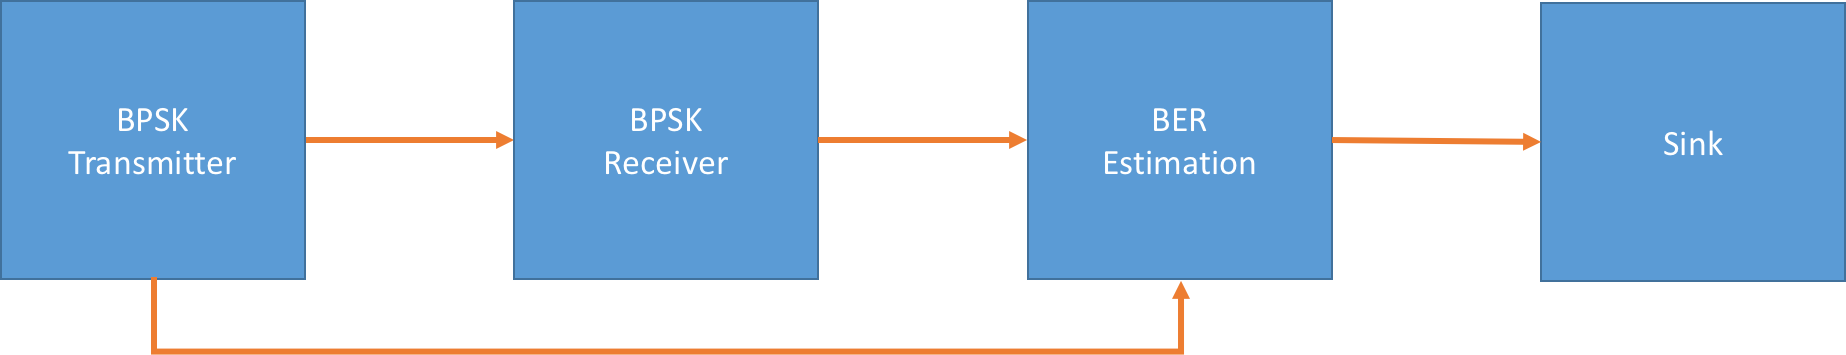
\includegraphics[width=\linewidth]{bpskdiagram.png}
\caption{Overview of the BPSK system being simulated.}
\label{fig:homodynesystem}
\end{figure}

\begin{table}[H]
\centering
\begin{tabular}{c|c}
System Blocks    & netxpto Blocks   \\ \hline
BPSK Transmitter & MQamTransmitter  \\
BPSK Receiver    & HomodyneReceiver \\
BER Estimator    & BitErrorRate
\end{tabular}
\end{table}

\subsection*{Required files}\label{Required files}

Header Files

\begin{table}[H]
\centering
\begin{tabulary}{1.0\textwidth}{|L|L|}
\hline
\textbf{File}            & \textbf{Description} 				                  \\ \hline
netxpto.h                & Generic purpose simulator definitions.	              \\ \hline
m\_qam\_transmitter.h    & Generates the signal with coded constellation.       \\ \hline
homodyne\_reciever.h     & Performs coherent detection on the input signal.     \\ \hline
sampler.h                & Samples the input signal at a user defined frequency. \\ \hline
bit\_decider.h           & Decodes the input signal into a binary string.       \\ \hline
bit\_error\_rate.h       & Calculates the bit error rate of the decoded string. \\ \hline
sink.h                   & Closes any unused signals.                           \\ \hline
\end{tabulary}
\end{table}		
%
Source Files
\begin{table}[H]
\centering
\begin{tabulary}{1.0\textwidth}{|L|L|}
\hline
\textbf{File}              & \textbf{Description} 					             \\ \hline
netxpto.cpp                & Generic purpose simulator implementations.           \\ \hline
m\_qam\_transmitter.cpp    &  Generates the signal with coded constellation.      \\ \hline
homodyne\_reciever.cpp     & Performs coherent detection on the input signal.     \\ \hline
sampler.cpp                & Samples the input signal at a user defined frequency. \\ \hline
bit\_decider.cpp           & Decodes the input signal into a binary string.       \\ \hline
bit\_error\_rate.cpp       & Calculates the bit error rate of the decoded string. \\ \hline
sink.cpp                   & Closes any unused signals.                           \\ \hline
\end{tabulary}
\end{table}		

\subsection*{System Input Parameters}

This system takes into account the following input parameters:

\begin{table}[H]
\centering
\begin{tabulary}{1.0\textwidth}{|C|C|}
\hline
\textbf{System Parameters} & \textbf{Description} 																 \\ \hline
numberOfBits               & Gives the number of bits to be simulated		          										 \\ \hline  
bitPeriod                  & Sets the time between adjacent bits                                                           \\ \hline 
samplesPerSymbol           & Establishes the number of samples each bit in the string is given 	         \\ \hline
pLength                    & PRBS pattern length					                      									 \\ \hline  
iqAmplitudesValues         & Sets the state constellation																	 \\ \hline  
outOpticalPower\_dBm       & Sets the optical power, in units of dBm, at the transmitter output							 \\ \hline  
loOutOpticalPower\_dBm     & Sets the optical power, in units of dBm, of the local oscillator used in the homodyne detector \\ \hline  
localOscillatorPhase       & Sets the initial phase of the local oscillator used in the homodyne detector					 \\ \hline  
transferMatrix             & Sets the transfer matrix of the beam splitter used in the homodyne detector					 \\ \hline  
responsivity               & Sets the responsivity of the photodiodes used in the homodyne detector						 \\ \hline  
amplification              & Sets the amplification of the trans-impedance amplifier used in the homodyne detector			 \\ \hline  
noiseAmplitude             & Sets the amplitude of the gaussian thermal noise added in the homodyne detector				 \\ \hline  
delay                      & Sets the delay factor of the homodyne detector												 \\ \hline  
posReferenceValue          & \multirow{2}{*}{Set the positive and negative reference values for the bit decision block}     \\ \cline{1-1}
negReferenceValue          &                                                                                                \\ \hline
confidence                 & Sets the confidence interval for the calculated QBER                                           \\ \hline  
midReportSize              & Sets the number of bits between generated QBER mid-reports                                     \\ \hline                   
\end{tabulary}
\end{table}		

\subsection*{Inputs}

This system takes no inputs.

\subsection*{Outputs}

This system outputs the following objects:
\begin{itemize}
\item Signals:
\begin{itemize}
\item Initial Binary String; (S$_0$)
\item Optical Signal with coded Binary String; (S$_{1}$)
\item Local Oscillator Optical Signal; (S$_{2}$)
\item Beam Splitter Outputs; (S$_{3}$, S$_{4}$)
\item Homodyne Detector Electrical Output; (S$_{5}$)
\item Decoded Binary String; (S$_{6}$)
\item BER result String; (S$_{7}$)
\end{itemize}
\item Other:
\begin{itemize}
\item Bit Error Rate report in the form of a .txt file. (BER.txt)
\end{itemize}
\end{itemize}

\subsection*{Simulation Results}

The following results show the dependence of the error rate with the signal power assuming a constant Local Oscillator power of $-20~dBm$. For reference, the eye diagram at 3 different power levels are also presented. The full line represents the expected results, note that it has been computed assuming a gaussian distribution of the thermal noise, which is not exact given the effect of the matched filter applied before the decoding of the bits, this explains the deviation between the simulation results and the expected values.

\begin{figure}[H]
\centering
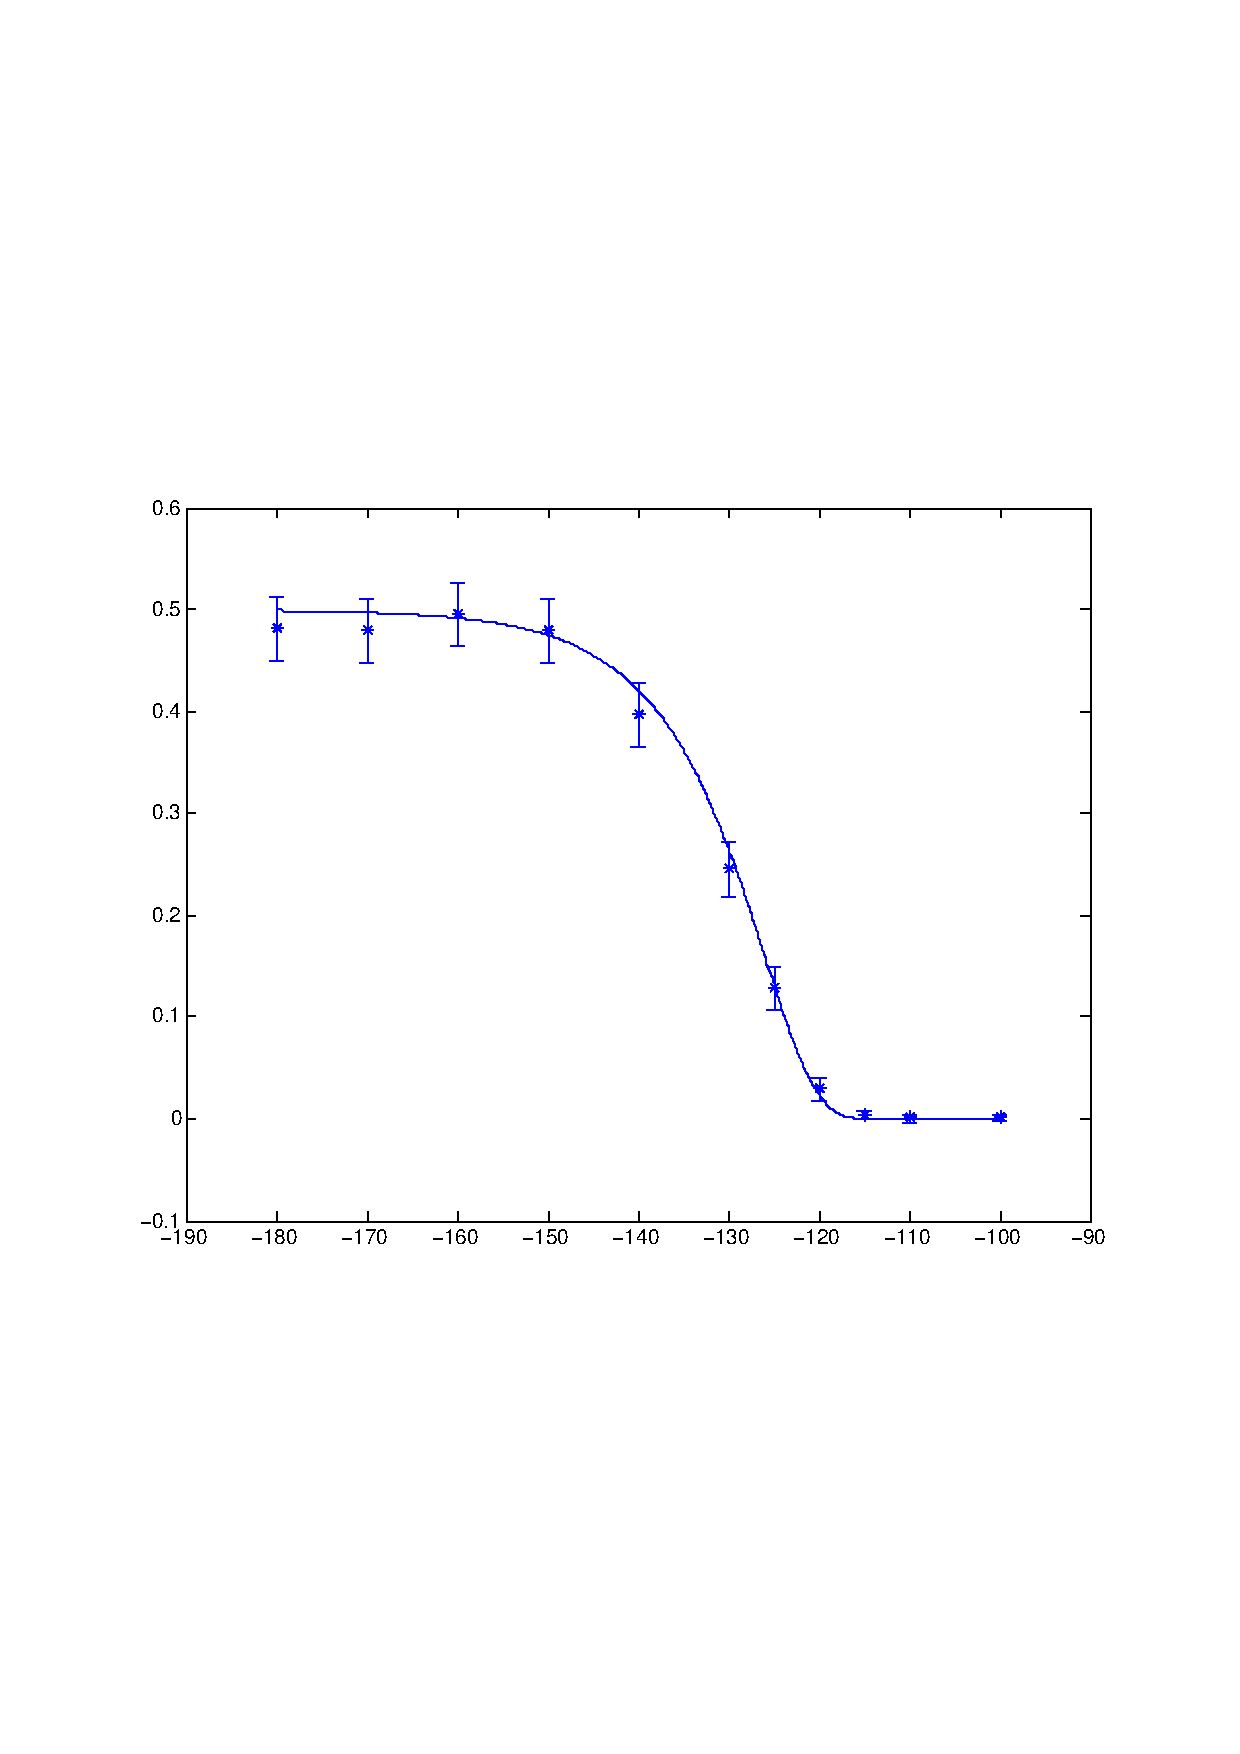
\includegraphics[width=\linewidth, trim= 0mm 85mm 0mm 85mm, clip]{berevolution.pdf}
\caption{Bit Error Rate in function of the signal power in dBm.}
\label{fig:berevolution}
\end{figure}

\begin{figure}[H]
\centering
\begin{subfigure}{.3\linewidth}
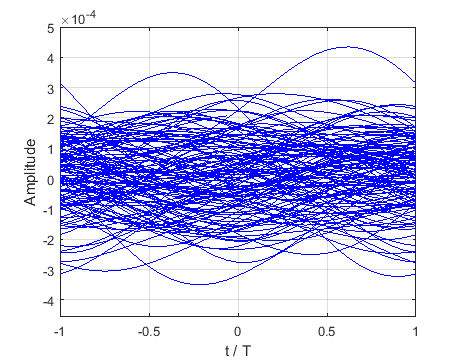
\includegraphics[width=\linewidth]{eyeclosed.png}
\caption{Power=-180dBm}
\end{subfigure}
\begin{subfigure}{.3\linewidth}
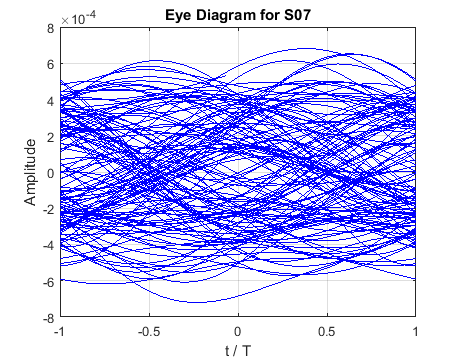
\includegraphics[width=\linewidth]{eyepartial.png}
\caption{Power=-130dBm}
\end{subfigure}
\begin{subfigure}{.3\linewidth}
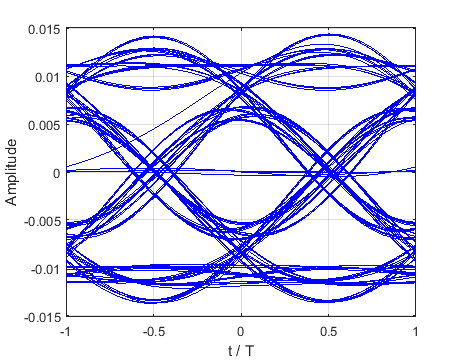
\includegraphics[width=\linewidth]{eyeopen.png}
\caption{Power=-100dBm}
\end{subfigure}
\caption{Eye diagrams at different signal powers.}
\end{figure}


%\section{Simulation Results}
%
%We consider the following scenarios:
%\begin{itemize}
%\item \ref{subsec:scenario1} Basic BPSK back to back with  thermal noise.
%\end{itemize}
%
%\subsection{BPSK with thermal noise}\label{subsec:scenario1}
%
%The following results were obtained from the simulation using the following input parameters:
%\begin{table}[H]
%\centering
%\begin{tabular}{rl}
%numberOfBits=           & 1000                                                     \\
%samplesPerSymbol=       & 16                                                       \\
%pLength=                & 5                                                        \\
%iqAmplitudesValues=     & \{ \{ 1, 0 \}, \{ -1, 0 \} \}                            \\
%outOpticalPower\_dBm=   & -20                                                      \\
%loOutOpticalPower\_dBm= & -10                                                      \\
%localOscillatorPhase=   & 0                                                        \\
%transferMatrix=         & \{ \{ 1/sqrt(2), 1/sqrt(2), 1/sqrt(2), -1/sqrt(2) \} \}  \\
%responsivity=           & 1                                                        \\
%amplification=          & 1e6                                                      \\
%noiseAmplitude=         & 15.397586549153788                                       \\
%delay=                  & 9                                                        \\
%\end{tabular}
%\end{table}
%
%The system took the binary string presented in Figure~\ref{fig:sentkey} and encoded it into the optical signal in Figure~\ref{fig:sentsig}. Notice the BPSK constelation of the signal, presented in Figure~\ref{fig:constellation}.
%\begin{figure}[H]
%\centering
%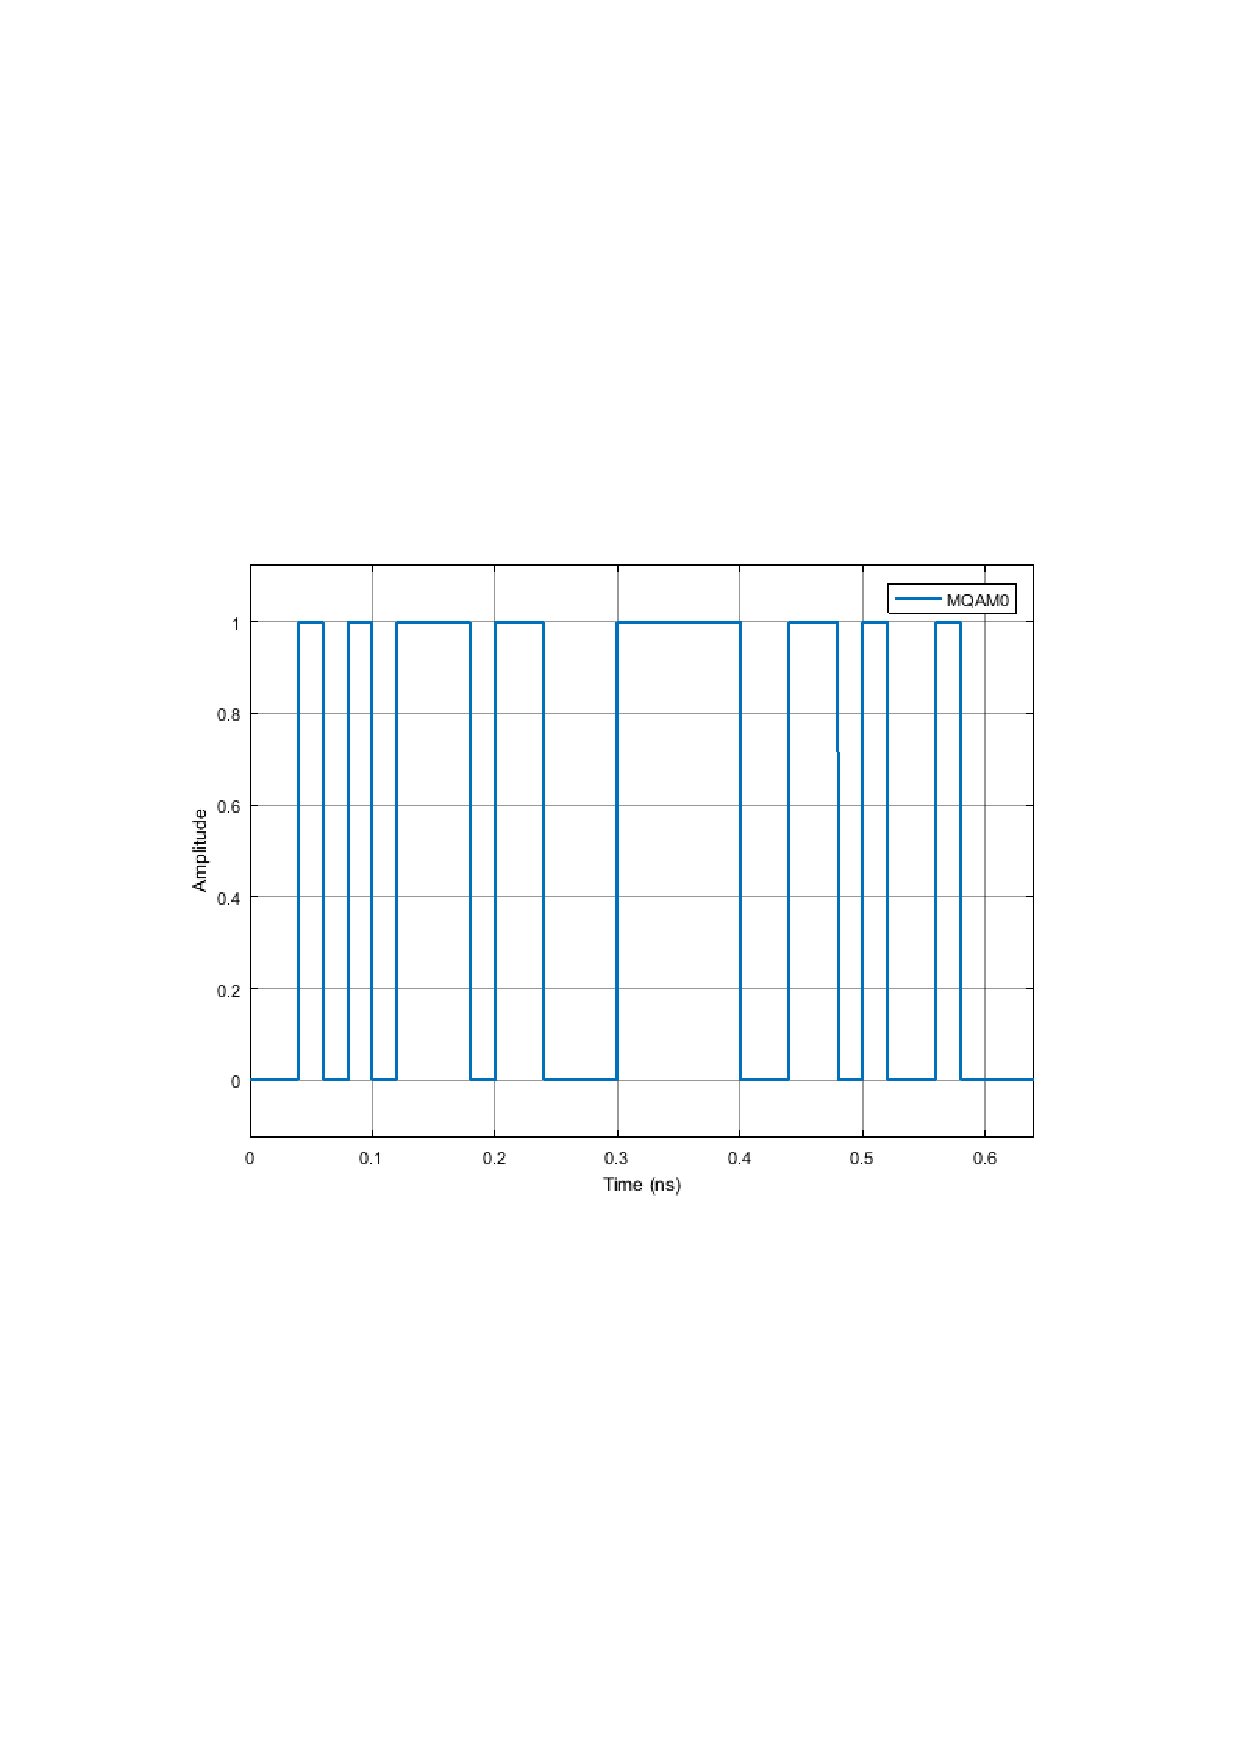
\includegraphics[width=\linewidth, trim= 0mm 95mm 0mm 95mm, clip]{binarystring.pdf}
%\caption{Sent binary key.}
%\label{fig:sentkey}
%\end{figure}
%
%\begin{figure}[H]
%\centering
%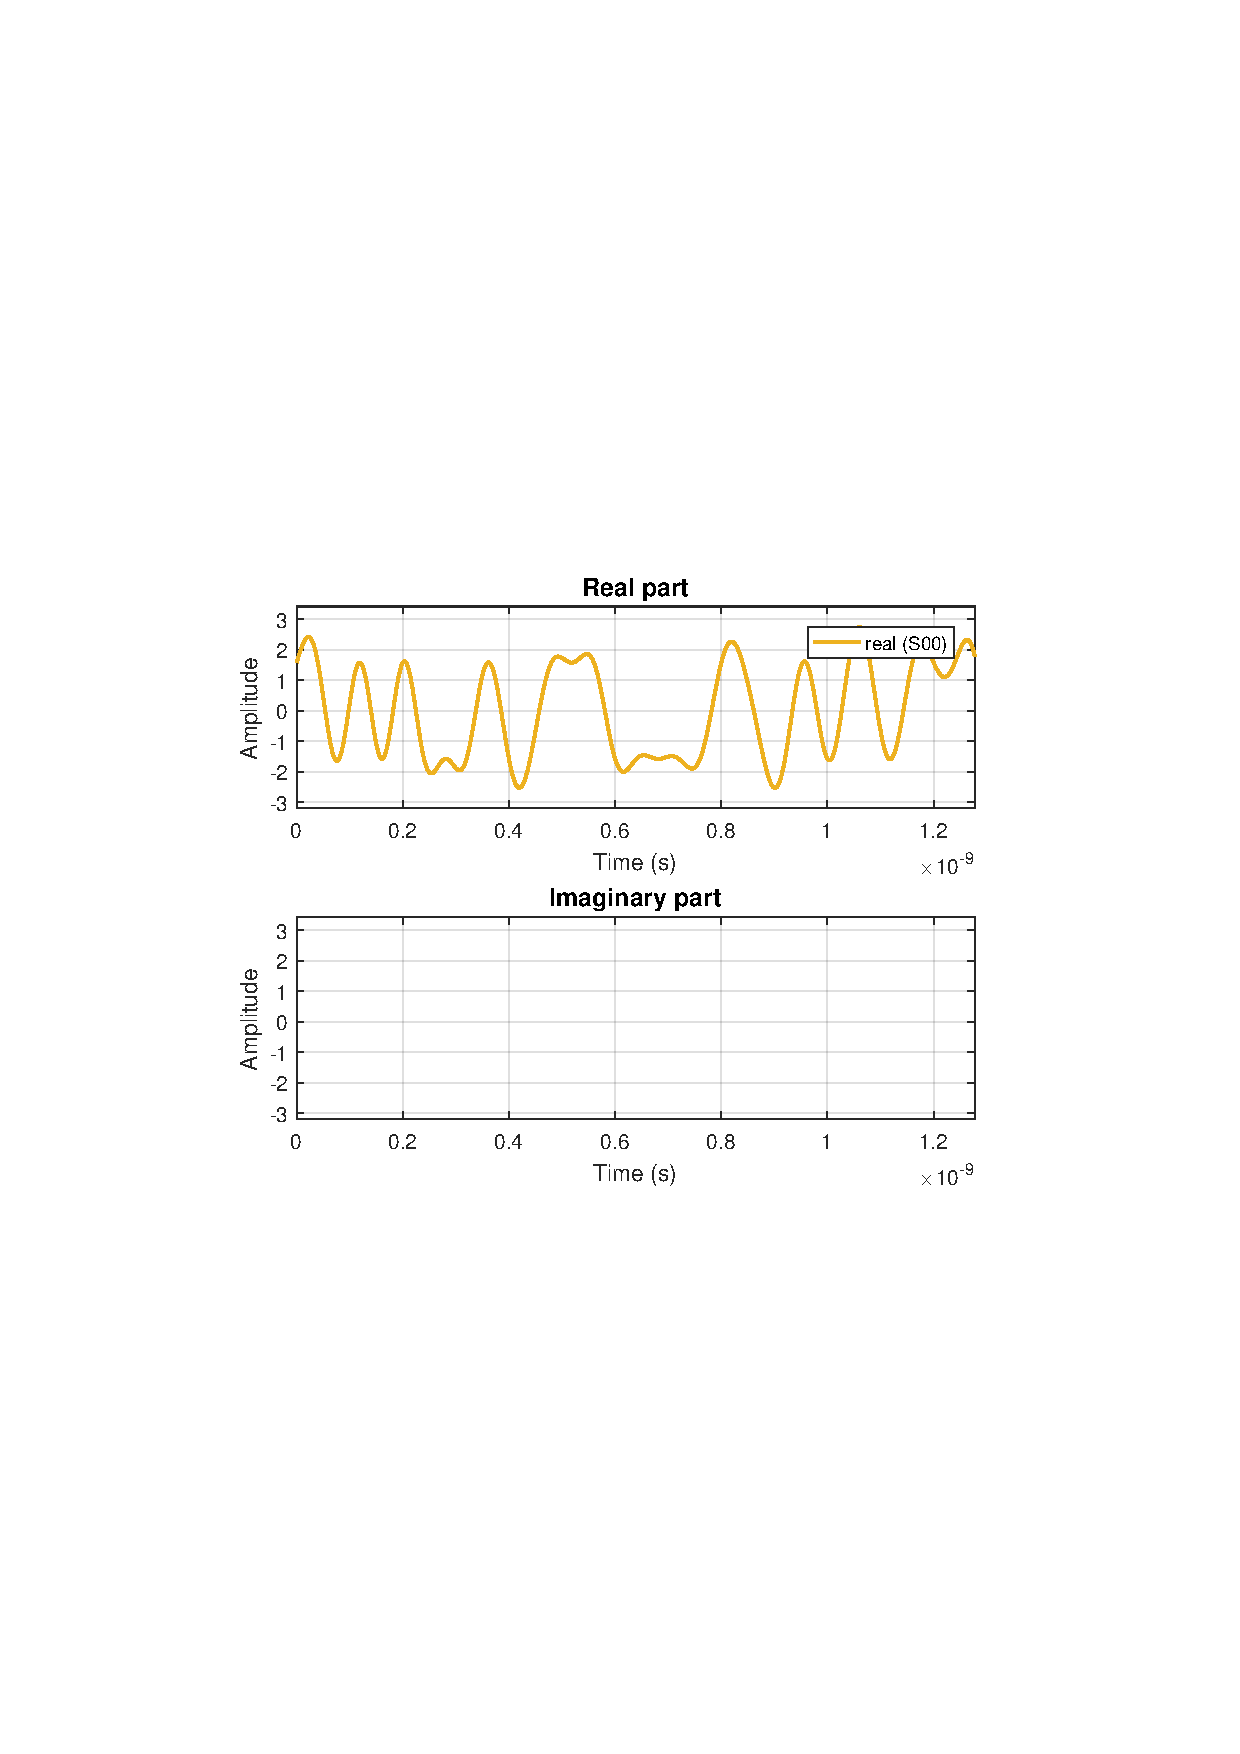
\includegraphics[width=\linewidth, trim= 0mm 95mm 0mm 95mm, clip]{sentsignal.pdf}
%\caption{Sent signal.}
%\label{fig:sentsig}
%\end{figure}
%
%\begin{figure}[H]
%\centering
%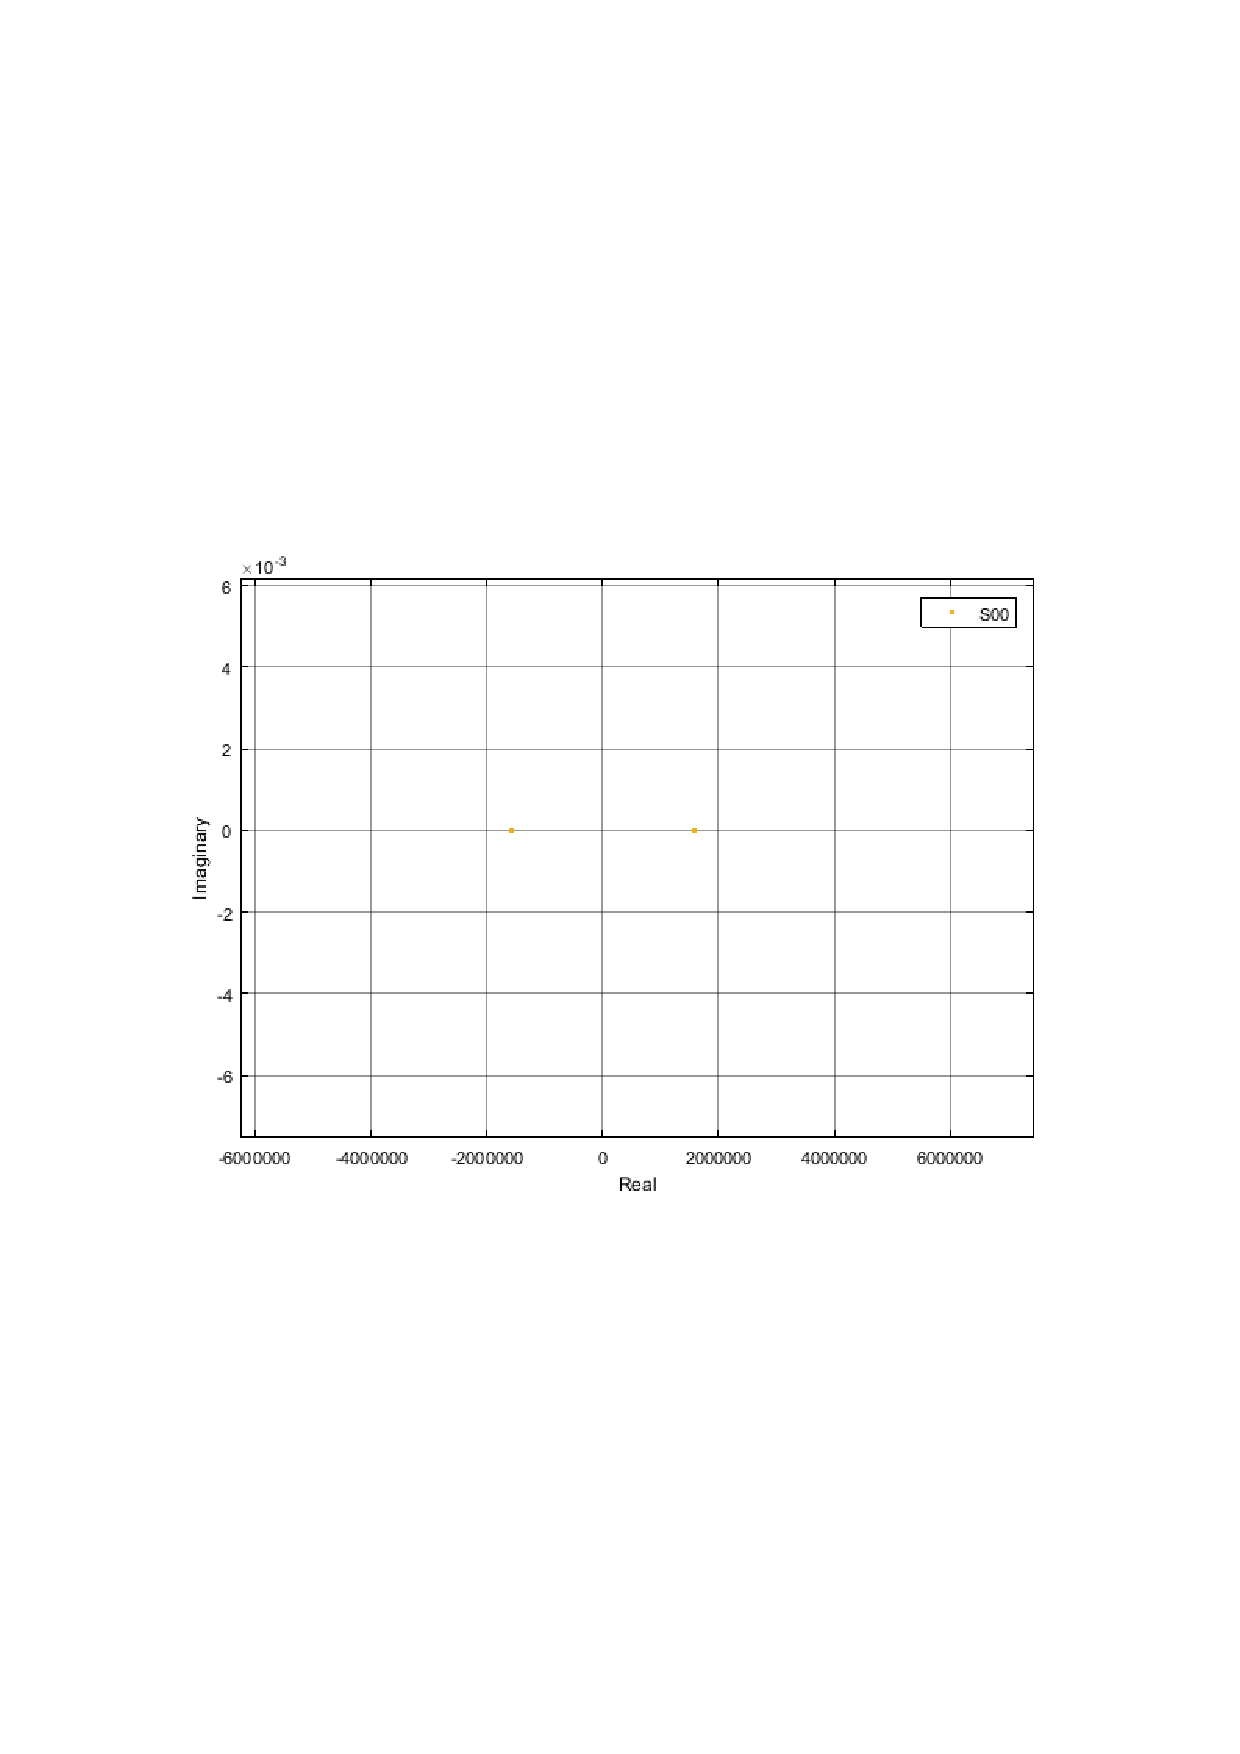
\includegraphics[width=\linewidth, trim= 0mm 95mm 0mm 95mm, clip]{constellation.pdf}
%\caption{Constellation of the sent signal.}
%\label{fig:constellation}
%\end{figure}
%
%Homodyne detection is then performed, using to that effect the local oscillator signal presented in Figure~\ref{fig:local}. Figures~\ref{fig:subtract}~and~\ref{fig:noisy} show the addition of noise to the signal.

%\begin{figure}[H]
%\centering
%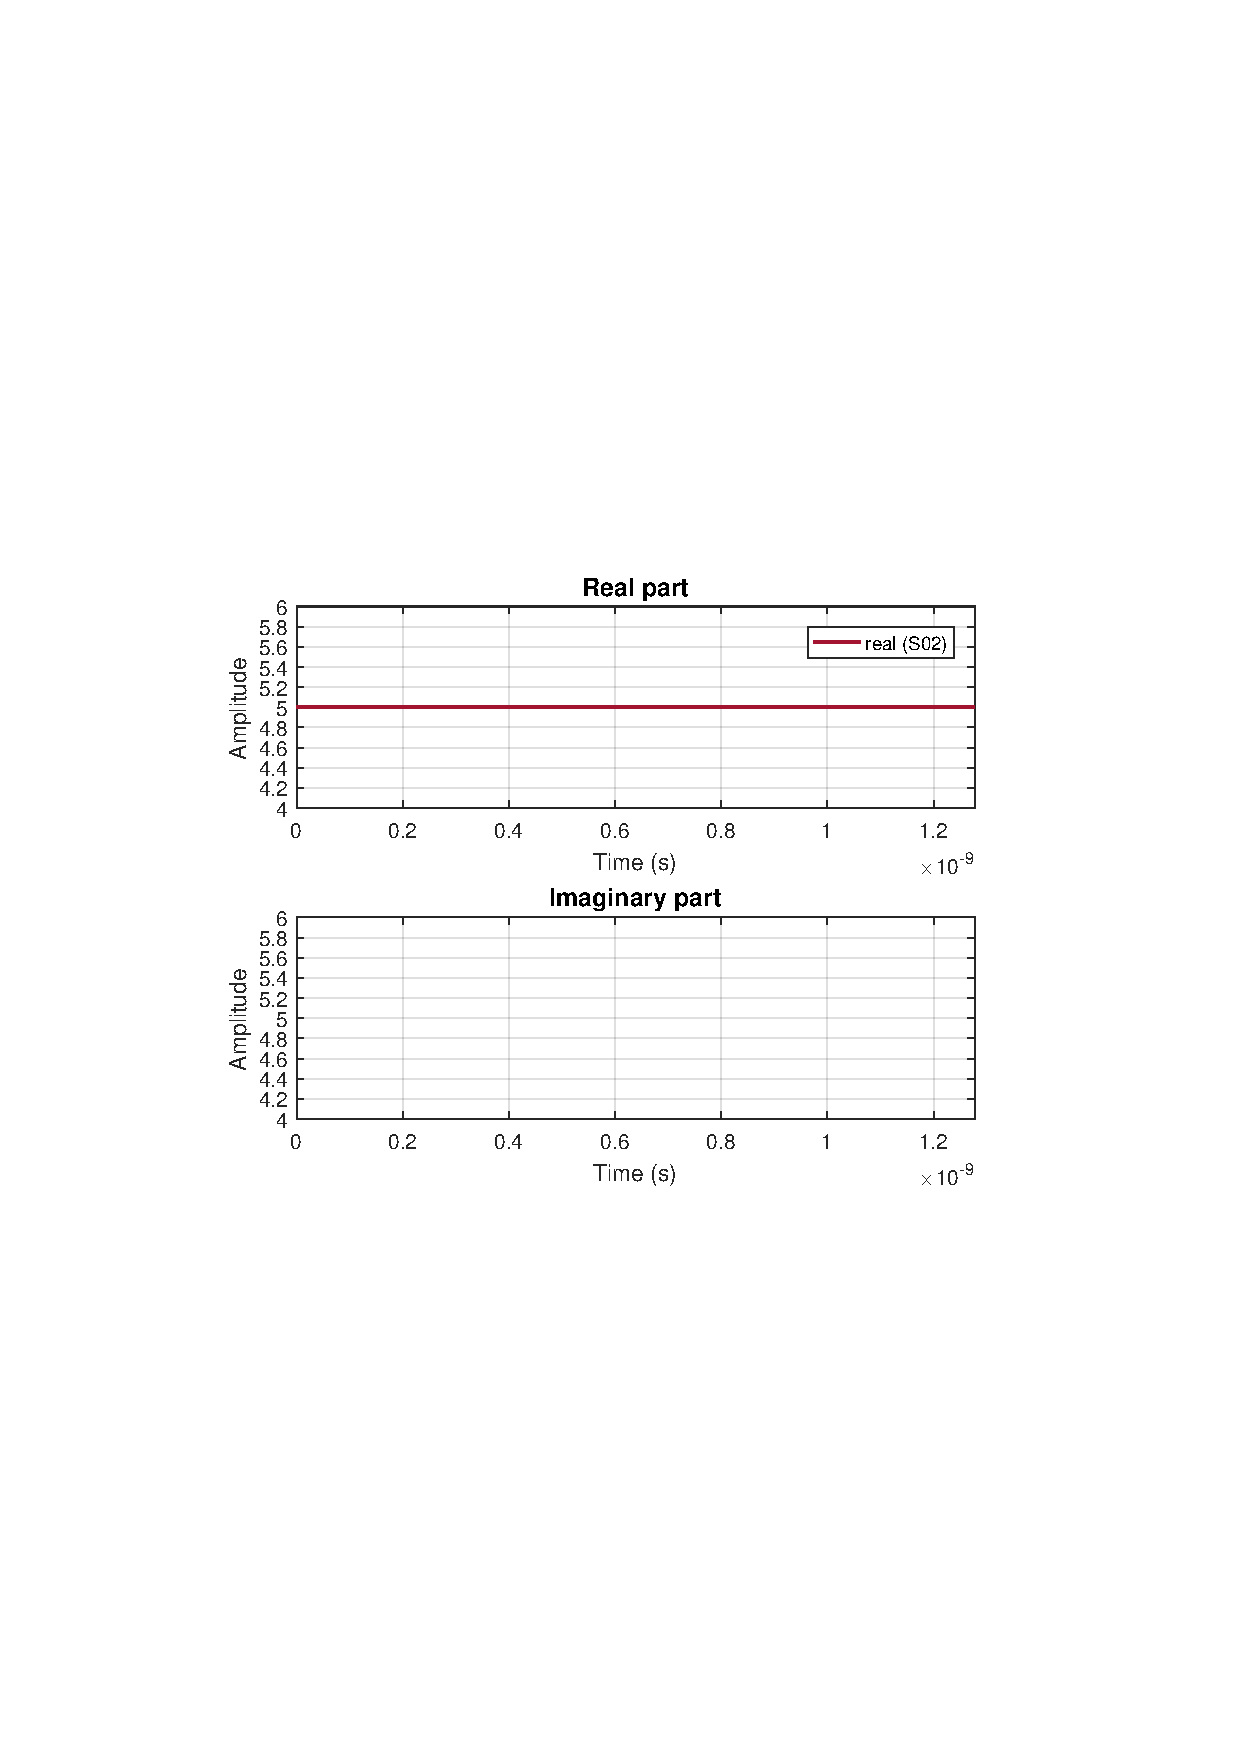
\includegraphics[width=\linewidth, trim= 0mm 95mm 0mm 95mm, clip]{localosc.pdf}
%\caption{Homodyne receiver internal signal: local oscillator used for Homodyne detection.}
%\label{fig:local}
%\end{figure}
%
%\begin{figure}[H]
%\centering
%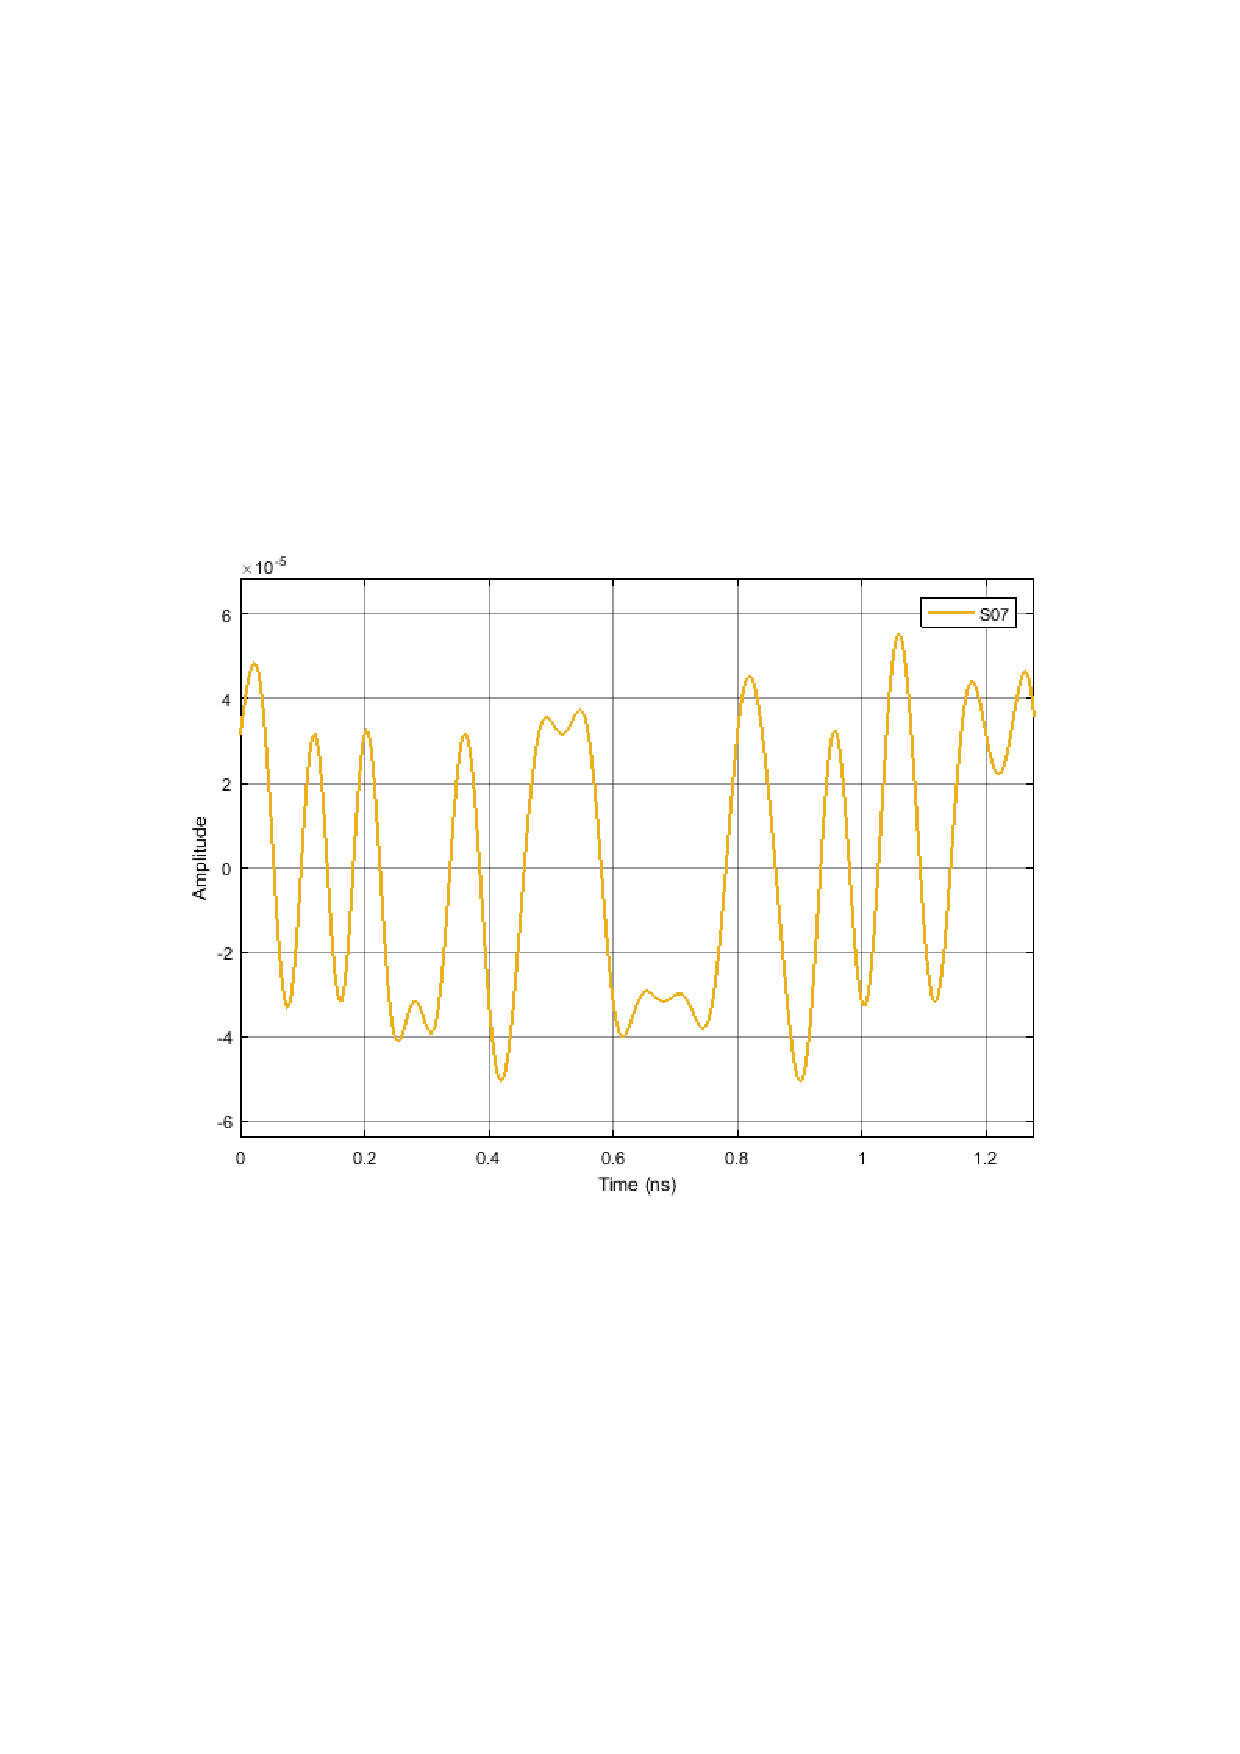
\includegraphics[width=\linewidth, trim= 0mm 95mm 0mm 95mm, clip]{subtract.pdf}
%\caption{Homodyne receiver internal signal: subtraction of the signals outputted by the photodiodes.}
%\label{fig:subtract}
%\end{figure}

%\begin{figure}[H]
%\centering
%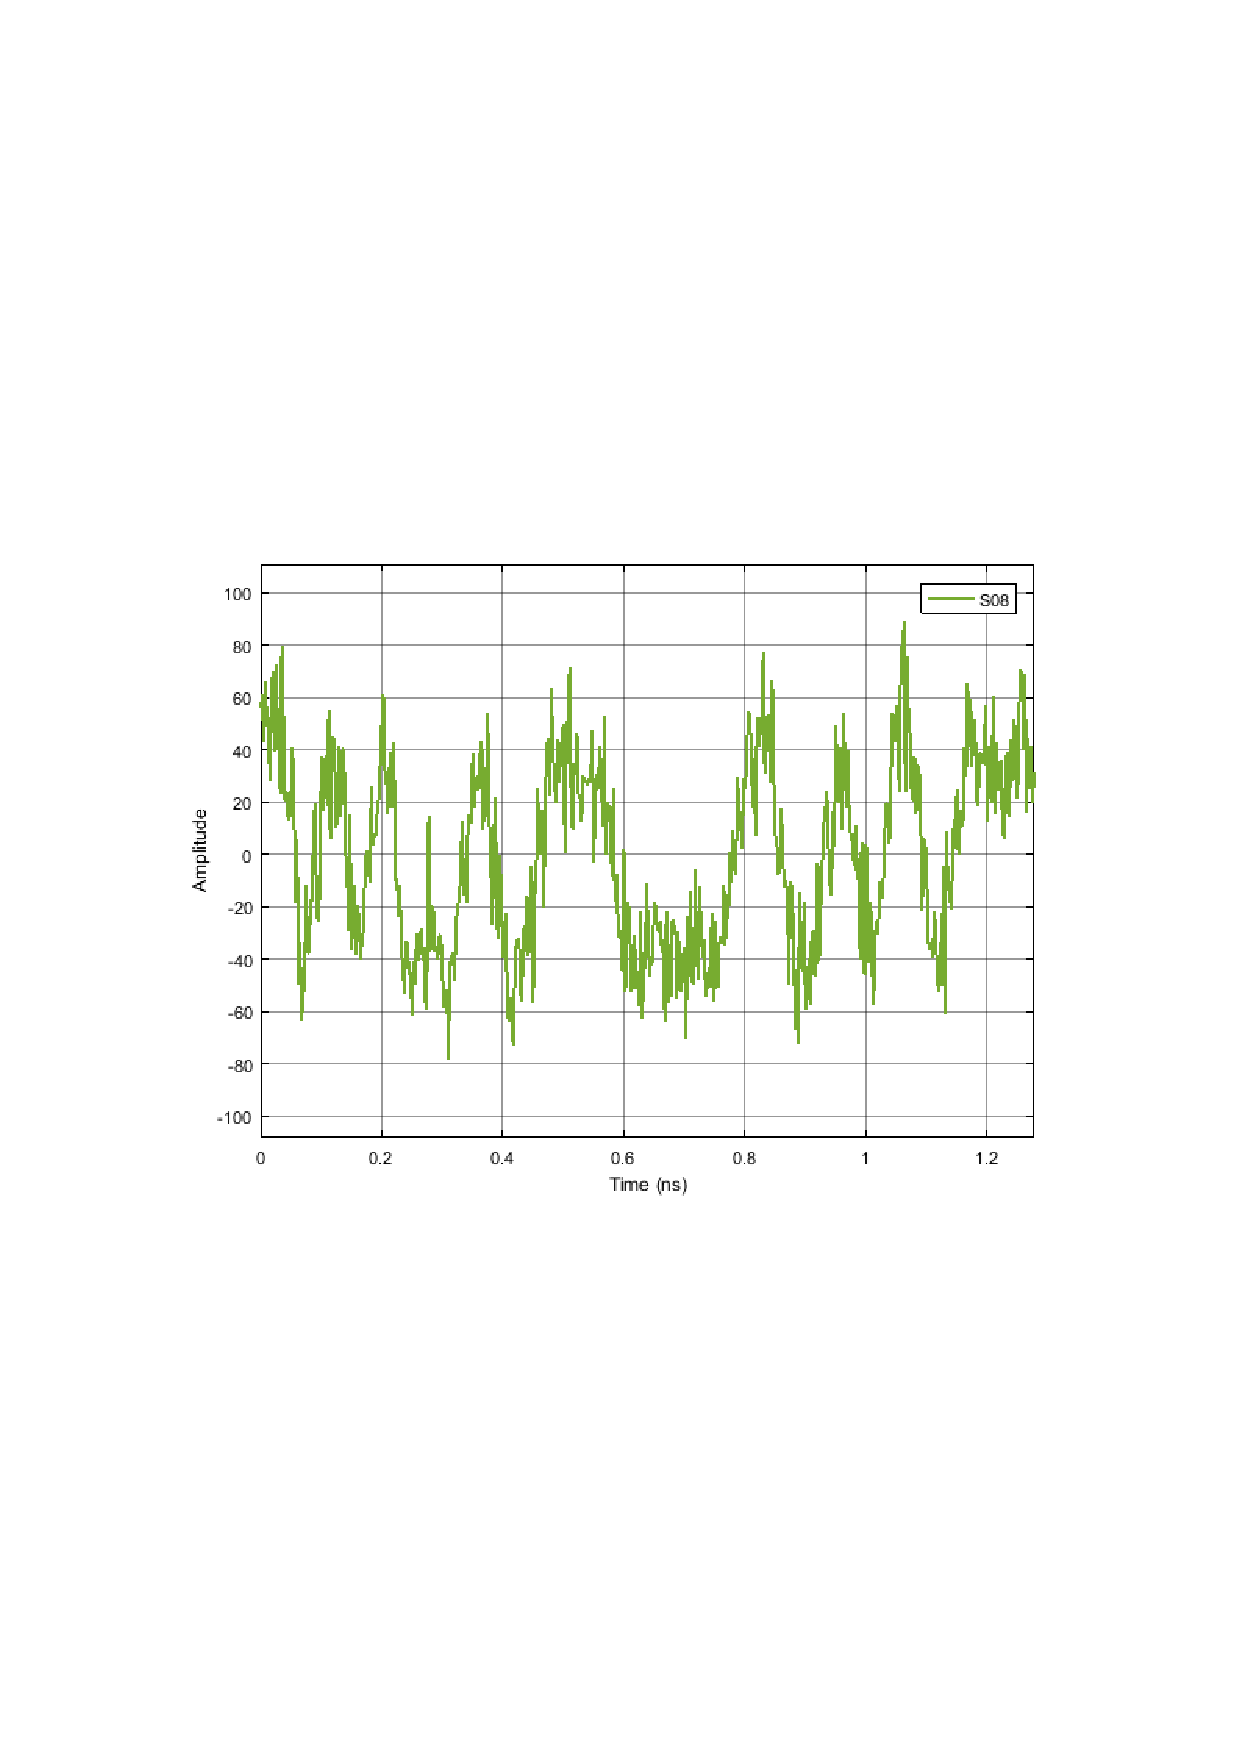
\includegraphics[width=\linewidth, trim= 0mm 95mm 0mm 95mm, clip]{noisy.pdf}
%\caption{Homodyne receiver internal signal: amplification of the signal in Figure~\ref{fig:subtract} with added noise.}
%\label{fig:noisy}
%\end{figure}

%The result of the homodyne detection is the binary string presented in~\ref{fig:decoded}, which is then compared to the original binary string by the BER block, which outputs the report presented in Figure~\ref{fig:ber}.
%
%\begin{figure}[H]
%\centering
%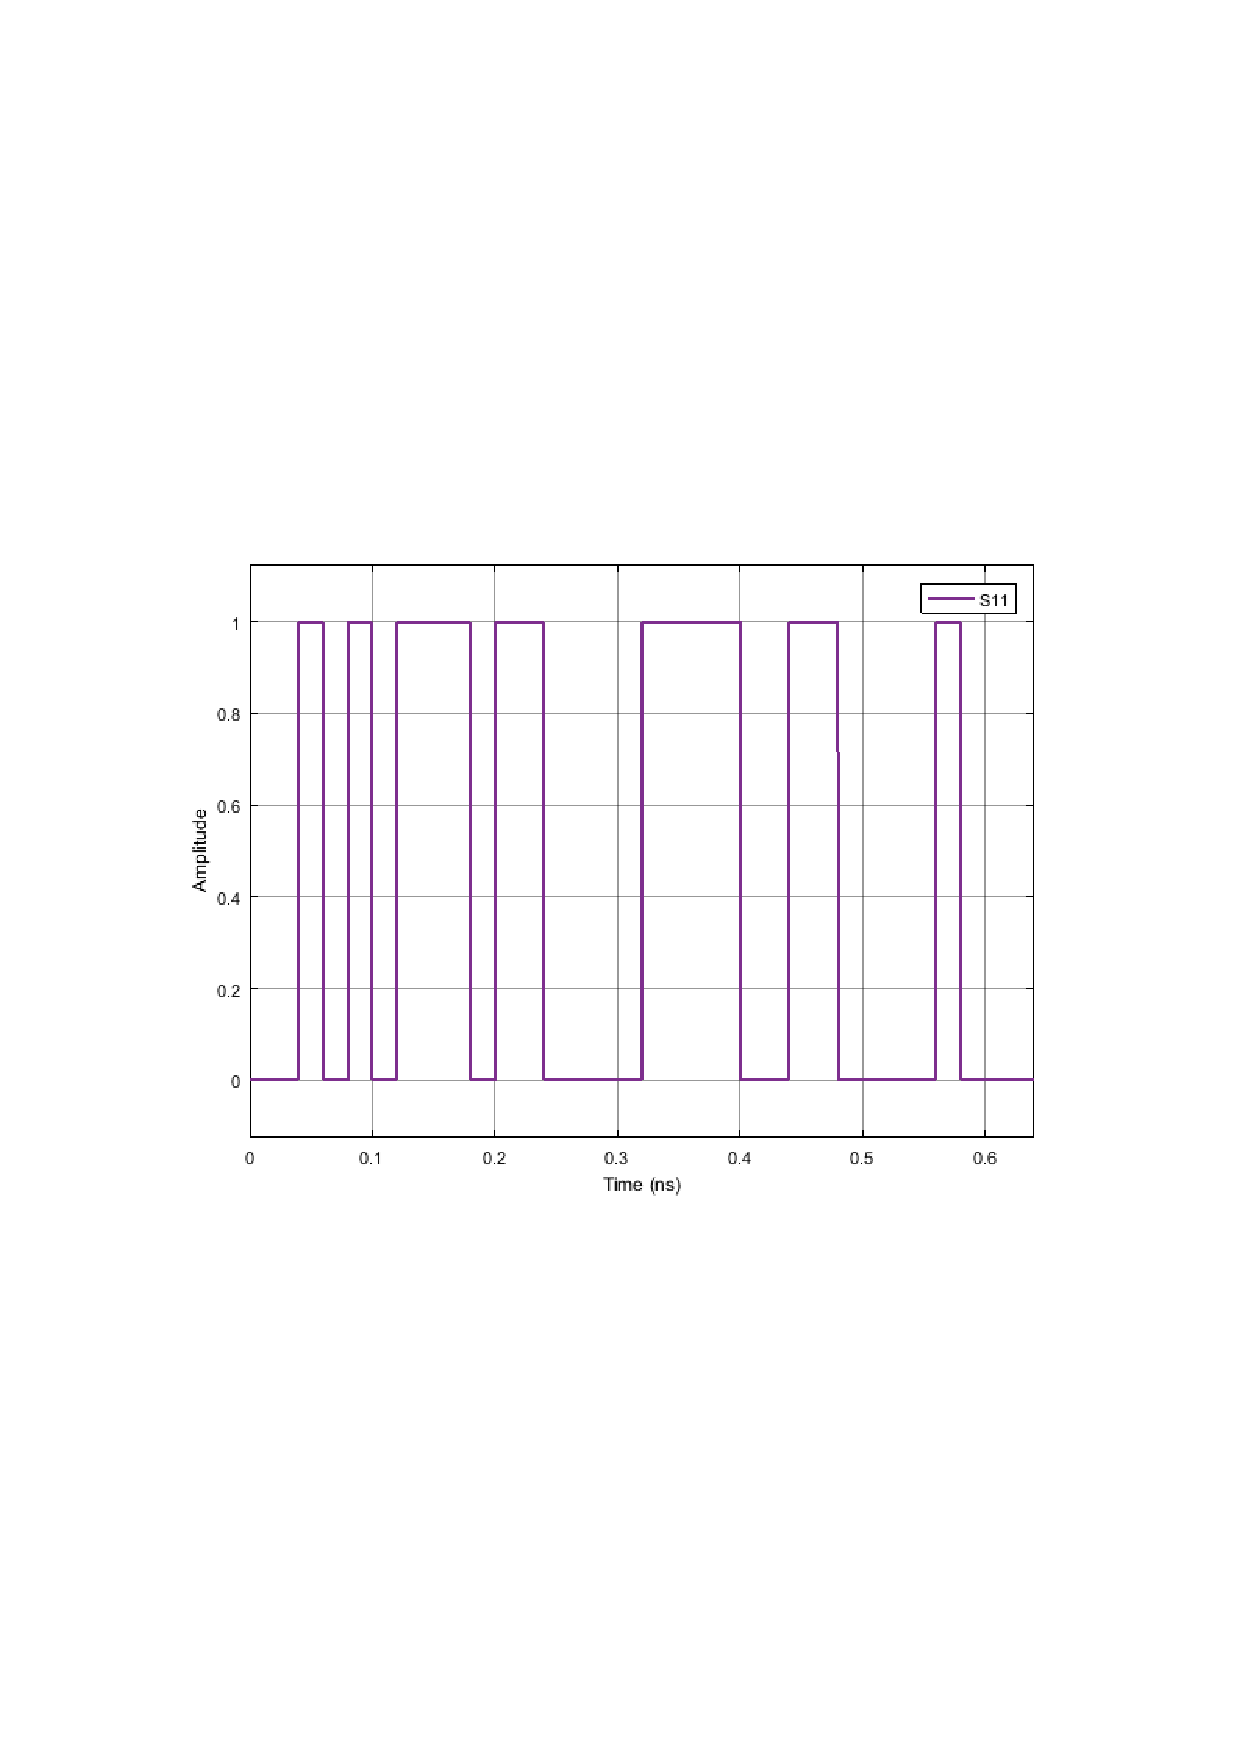
\includegraphics[width=\linewidth, trim= 0mm 95mm 0mm 95mm, clip]{decodedbinarystring.pdf}
%\caption{Decoded binary string, output of the Homodyne receiver block.}
%\label{fig:decoded}
%\end{figure}

%\begin{figure}[H]
%\centering
%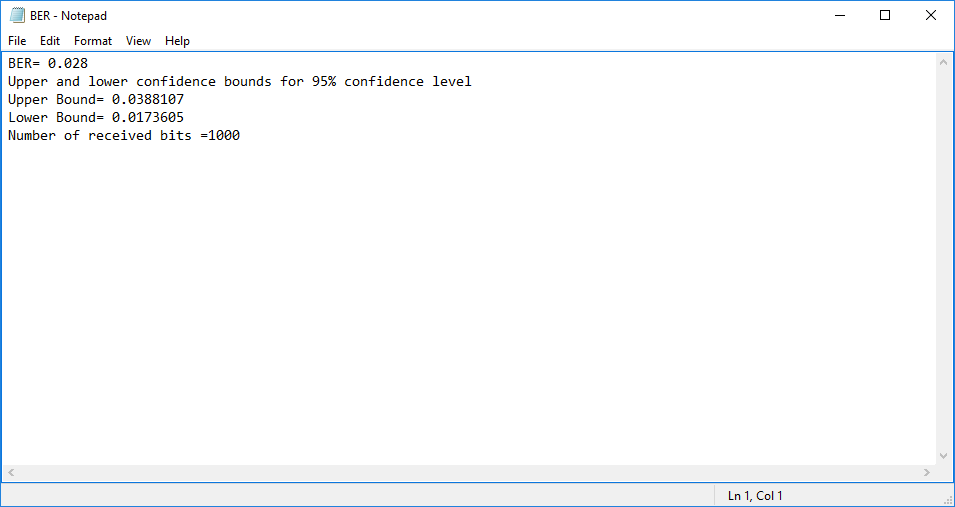
\includegraphics[width=\linewidth]{berreport.png}
%\caption{Bit-Error-Rate report.}
%\label{fig:ber}
%\end{figure}



%\section{Block Description}

%\subsection{MQAM Transmitter}
%% subfile goes here
%
%\subsection{Homodyne Receiver}
%\subfile{../../lib/tex/i_homodyne_reciever}
%
%
%\subsection{Bit Error Rate}
%\subfile{../../lib/tex/ber}
%
%\subsection{Local Oscillator}
%\subfile{../../lib/tex/localoscillator}
%
%\subsection{Beam Splitter}
%\subfile{../../lib/tex/beamsplitter}
%
%\subsection{Photodiode}
%\subfile{../../lib/tex/photodiode}
%
%\subsection{Amplifier}
%\subfile{../../lib/tex/ideal_amplifier}
%
%\subsection{Electrical Filter}
%\subfile{../../lib/tex/pulse_shaper}
%
%\subsection{Sampler}
%\subfile{../../lib/tex/sampler}
%
%\subsection{Bit Decider}
%\subfile{../../lib/tex/decider}
%
%\subsection{Bit Error Rate}
%\subfile{../../lib/tex/ber}

%\section{Known Problems}
%\begin{enumerate}
%    \item{Finish section~\ref{Required files} of this document.}
%    \item{Change figure 1 to increase the lines width and to include the block Sink, and to include the signals names S0, S1, S2, S3.}
%    \item Homodyne Super-Block not functioning
%    \item MQAM Transmitter PDF needs to be written
%    \item 8 bits being lost of every signal
%    \item If the bit string length is larger than 512, this first 512 bits are lost
%\end{enumerate}

\end{document} 